\documentclass{standalone}
\usepackage{tikz}
\usetikzlibrary{arrows.meta, decorations.markings, intersections, positioning}

\begin{document}
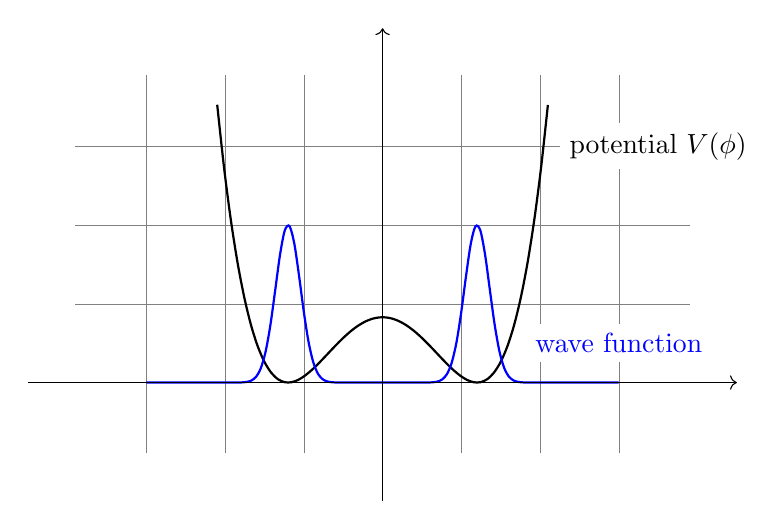
\begin{tikzpicture}

\def\a{1.2}
\def\b{.4}
\def\c{20}
\def\d{2}

\draw[gray, very thin, step=1] (-3.9,-.9) grid[] (3.9,3.9);

\draw[thick] plot[smooth, samples=50, domain=-2.1:2.1] (\x, {\b * (\x*\x - \a*\a)*(\x*\x - \a*\a)});

\draw[blue, thick] plot[smooth, samples=100, domain=-3:3] 
    (\x, 
    {
        \d * exp(-\c * (\a-\x) * (\a-\x)) +
        \d * exp(-\c * (\a+\x) * (\a+\x))
    });

\node[fill=white] at (3.5,3) {potential $V(\phi)$};
\node[blue,fill=white] at (3,.5) {wave function};

\draw[ -> ] (-4.5,0) -- (4.5,0);
\draw[ -> ] (0,-1.5) -- (0,4.5);

\end{tikzpicture}
\end{document}